%!TEX root = main.tex

\section{Obsevations}

\boldification{here we report on how participants created and used context as they were working on their programming task.}
In this paper, we investigate how programmers create context of the programming task they are working on. For our purpose, we observed the types of artifacts that participant referred to perform different programming activity. Here we present the observation we draw from the participants? interactions with the artifacts while performing specific programming activities to understand how they created the context. Our focus was to build an understanding of how the context building process occurs, and gain insight into what factors play a role in forming this context. 

We didn?t restrict our observation to any medium, as context is a broad notion and anything around a person, from the placement of a paper to the color of the screen, can affect it. We also collected diverse data in the form or think aloud, screen capture, facial expression, video of workspace and any notes or diagrams the participants drew to recognize the subtle hints which may suggest that information was added to the context or obtained from the context. From these data, we identified the different types of artifact the participants use. 

Table~\ref{tab:programming-activities} presents the programming activity that P4 performs and the artifacts she interacts when performing the programming activities. The first column shows all the programming activities that P4 performed, out of the 12 activities discussed in Table 1 that we coded. The second column shows the frequency with which P4 accessed each type of artifact within each programming activity. The third column shows a breakdown of the artifacts for each type, with the frequency of each artifact shown as bar graphs. Artifact names have been anonymized for analysis purposes. 
**We identify the type of artifact and the specific instance of the artifact correlated with the type of programming activity to get a finer-grained understanding of what was used to create context. Table x...does this.

%!TEX root = ../main.tex

\begin{table*}
\caption{Programming activities and the most frequently accessed artifacts associated with them}
\label{tab:programming-activities}
\begin{tabular}{lll}
\toprule
Programming Activity & Artifact type [frequency] & Artifact type frequencies for each type \\
\midrule
\multirow{3}{*}{A0 - Coding} & Code [32] & [2,6,5,4,12,2,1] \\
& Tools [12] & [1, 1,5,1,3,1] \\
& Documents [2] & [2] \\
\midrule
\multirow{2}{*}{A1 - Interaction with documents} & Documents [19] & [19] \\
& External Artifacts [20] & [13,7] \\
\midrule
\multirow{2}{*}{A2 - Navigation} & Code [9] & [0,1,1,0,5,1,1] \\
& Tool [1] & [0,0,1,0,0,0] \\
\midrule
\multirow{2}{*}{A4 - Reading Task Prompt} & Documents [22] & [22] \\
& External Artifacts [15] & [10,5] \\
\midrule
\multirow{2}{*}{A5 - Searching in web/IDE} & Code [4] & [0,0,1,1,2,0,0] \\
& Tool [1] & [0,0,1,0,0,0] \\
\midrule
\multirow{2}{*}{A6 - Reading Search Results} & Code [1] & [0,0,0,0,1,0,0] \\
& Web Resource & [1] \\
\midrule
\multirow{2}{*}{A7 - Processing Search Results} & Code [2] & [0,0,0,0,2,0,0] \\
& Web Resource & [1] \\
\midrule
\multirow{2}{*}{A8 - Viewing Web Resource} & Code [1] & [0,0,0,0,1,0,0] \\
& Web Resource & [1] \\
\midrule
A9 - Debugging & Code [1] & [0,0,0,0,1,0,0] \\
\midrule
\multirow{2}{*}{A11 - Idle} & Documents [2] & [2] \\
& External Artifacts & [1,1] \\
\bottomrule
\end{tabular}
\end{table*}

We saw 6 different types of artifacts - codefiles (.js, .java, etc.), documents (task description, requirements documentation), IDE tools (New class dialog box, getter-setter dialog box, terminal/console etc.), web resources (google search results, Stack-Overflow pages, api documentations), externalized artifacts (notes, diagrams, etc.), and other (calculators, project setup dialog box).

There are 7 code files (which we coded as c1.java, c2.java, ... , c7.java) that P4 created and worked with iteratively during the observational session. She used 6 IDE tools (t1, t2,..., t6) and referred to 1 document (d1) during this time. However, she also referred to 2 web sources (coded as w1 and w2) and created two external artifacts on paper (ex1 and ex2) that she repeatedly referred to.

\boldification{Same artifacts used across different activities}
\boldification{Participants accessed same artifacts for many different purposes (different aspects of programming). We find that the same artifacts were used to create context (understanding a problem, ideate) and apply context to form solution (form solution, code)**. For example?..in table x, we see?.}

We observed across different programming activities, participants accessed the same artifacts. We will talk about 2 examples here. From Table 2, P4 used the code file c5 12 times when she was coding [A0] and nine times when she was navigating. When we look closer, during the 60 minute session, all the navigations to c5 were not all for the purpose of coding. P4 coded [A0] in c5 for some time, moved to the requirements document [A4] and spent some time reading it. P4 briefly moved to c5 from the document, read through her code which we infer as an action to verify if her code meets the her design to meet the requirements. She went back to the requirements document [A4] and finally moved to the c5 file to start coding [A0] again.

On another instance, P4 moved from coding[A0] in c5 to searching on the web [A5] how to implement a certain concept, reading the search results [A6], choosing one that she perceived to be of highest value [A7] and finally reading the webpage she chose [A8]. She moved back and forth between the webpage w1 and the codefile c5 two times. Both times her cursor was on a part of the web page w1 which was a code snippet -- we inferred that she was checking for syntactical differences or errors. 

These observations reveal that the same artifacts are used across different programming activities.This contradicts the representational view of context, which suggest that ?context and activities are separable? [Dourish, Gasparic]. We see a difference in the type of artifacts across activities. Programming activity is an important aspect to consider when determining context. 


\boldification{Artifacts span Heterogeneous medium}
\boldification{**just a single view is not enough**}

\boldification{**yes code is the most frequent artifact when coding. But we see that outside of IDE a lot of stuff happened...so we need to have a broader aspect. Example [[pictures/ quotes]]}
It is true that, when working on a programming task, code files are most frequently accessed. P1 accessed three code files 87 times, P4 accessed seven code files 49 times and P6 accessed four code files 147 times during the one hour observation sessions.

However, participants also accessed resources on the website for learning how to use a concept/feature. The interactions with artifacts outside the IDE are also frequent with P6 accessing seven web resources 91 times. P6 uses a blog to learn how to use ?draggable? feature when he couldn?t get the desired function to work.

\boldification{**A lot of time, we saw people ideating and using stuff outside the computer too...this means context is broader than just online artifacts...and important to consider  and help developers capture?
We also observed that participants heavily engaged in creating external artifacts (like notes, diagrams etc.), communicating and ideating during these sessions. Figure 1 shows a plot of P1?s activities and the artifacts he interacts with for a segment of the session. From the plot, near the 22 minute mark, when P1 interacts with the code artifact c1, he was ideating while thinking aloud. However, his programming activities go from idle [A11] to communicating [A2] to selecting parts of the code as part of thinking aloud (marked as coding [A0]) and back to being idle [A11] in the IDE. }

\begin{figure*}
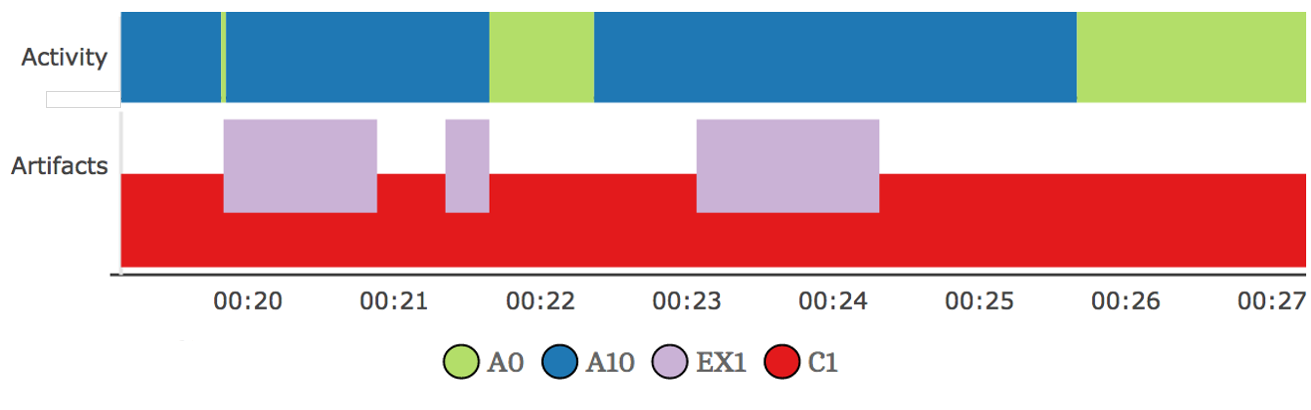
\includegraphics[width=\textwidth]{figures/P1timeplot}
\caption{Snippet of Activities and Artifacts from P1 (traffic prompt, 10-minute duration)}
\end{figure*}

This suggests that looking only at online (especially code) artifacts provide a tiny facet of what makes constitutes the whole process of context building during a programming task. During the interaction with web resources and periods of ideating, participants made progress towards solving the problem which they later implement. These non-IDE sources are factors that affect context, if not being part of the context itself.

\boldification{The programming activity guides interaction with the artifacts}
\boldification{**based on the activity, the interaction with artifacts change**}

When participants access the artifacts, the specific interactions with the artifacts -- selecting which part of the artifact to go to, whether they simply scroll through the artifact or highlight parts of the artifact, whether they copy text from these artifacts to paste into the code for debugging -- depends on the programming activity and the goal driving the activity. These differences are also observable through the difference in times spent on these artifacts.

Figure 2 shows the artifacts P6 accesses and the activities he performs. A marks the time P6 searched on the web to obtain the syntax for a javascript feature. The first time he reaches a Q and A webpage containing answers to his question (marked B) on the diagram, he scrolls through the first few answers before selecting one spending around 36 seconds. These interactions was driven by the goal to learn how to implement the feature for the purpose of coding [A0]. When his selected answer threw an error (marked as C), he went back to the web page and quickly scrolled and found the answer he had already identified (marked as D) and copies it to implement. This second visit to the webpage took only five seconds and was geared towards recalling the syntax for debugging purposes [A9]. 

Brandt et al [CITE] observed similar behavior in programmers where he was able to distinguish between the purposes of when programmers use online resources. He also found that participants spent the most time when learning from the web and least time when using the web to recall syntax.

\begin{figure*}
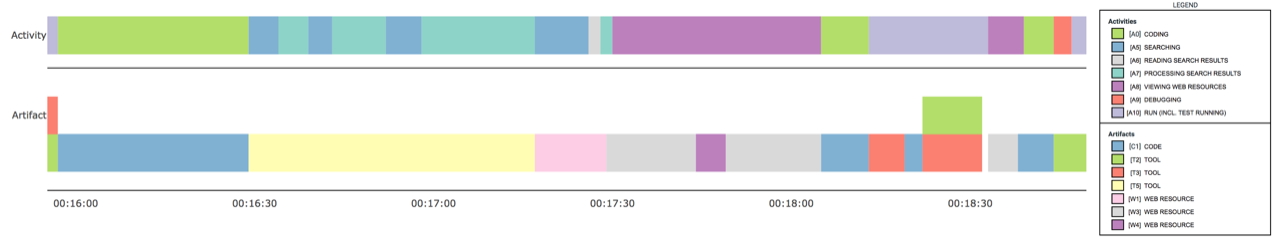
\includegraphics[width=\textwidth]{figures/P6timeplot}
\caption{Snippet of Activities and Artifacts from P6 (real-world development, 10-minute duration)}
\end{figure*}


\boldification{**memory plays a role - sequence matters [same activity, shorter time, memory plays role] [zoomed out figure]}

We also observe that memory plays a role in the interaction with artifacts. In the above example, across the different the coding [A0] and debugging [A9] activities, when P6 visited the webpage a second time it took him exactly five seconds to locate the syntax and copy it. We infer that in such a short amount of time, he could recall from his memory where the information was located. 

Across the three participants, we observe repeatedly, that participants recall information from memory to implement their goal. This 

\boldification{**Not only does context rise from the activity i.e. activity guides the specific type and amount of information obtained from the context/artifact, the activity was used to recall the relation between the context with which the artifacts were associated**}

\boldification{**this means that?.and is contrary to the assumptions of ?representational view of context, that context is stable and separate from activities? [...], is not what we see in our data. }

Interaction includes Reflection on the information gained from the artifacts:

\boldification{**Finally we see that, users conduct reflection/evaluation of the information they come across before deciding their next activity }
